\documentclass{article}
\usepackage[margin=1.0in]{geometry}
\usepackage{listings}
\usepackage{xcolor}
\usepackage{graphicx}
\usepackage{siunitx}
\usepackage{float}
\usepackage{setspace}
\usepackage{makecell}
\usepackage{gensymb}
\usepackage{url}
\usepackage{placeins}
\usepackage{caption}
\usepackage{inconsolata}
\usepackage{hyperref}

\title{ELEC 291 : Metal Detecting Robot}
\author{Team A9}
\date{April 12th, 2024}

\definecolor{codegreen}{rgb}{0,0.6,0}
\definecolor{codegray}{rgb}{0.5,0.5,0.5}
\definecolor{codepurple}{rgb}{0.58,0,0.82}
\definecolor{backcolour}{rgb}{0.95,0.95,0.92}

\lstdefinestyle{mystyle}{
    backgroundcolor=\color{backcolour},
    commentstyle=\color{codegreen},
    keywordstyle=\color{magenta},
    numberstyle=\tiny\color{codegray},
    stringstyle=\color{codepurple},
    basicstyle=\footnotesize\ttfamily,
    breakatwhitespace=false,
    breaklines=true,
    captionpos=b,
    keepspaces=true,
    numbers=left,
    numbersep=5pt,
    showspaces=false,
    showstringspaces=false,
    showtabs=false,
    tabsize=2
}

\linespread{1.6}
\setlength{\parindent}{0pt} % Disable paragraph indentation

\lstset{style=mystyle}

\begin{document}

\maketitle
\begin{center}
Course: ELEC 291/292 Electrical Engineering Design Studio I \\
Section: L2A \\
Instructor: Dr. Jesus Calvino-Fraga \\
\end{center}

\begin{center}
\begin{tabular}{|c|c|c|c|}
    \hline
    Student \# & Student Name & \%Points & Signature \\
    \hline
    67286750 & Tomaz Zlindra &  & 
\includegraphics[width = 1.5cm]{Names/Tomaz.jpeg}  \\
    \hline
    21475330 & Martin Lieu &  &
    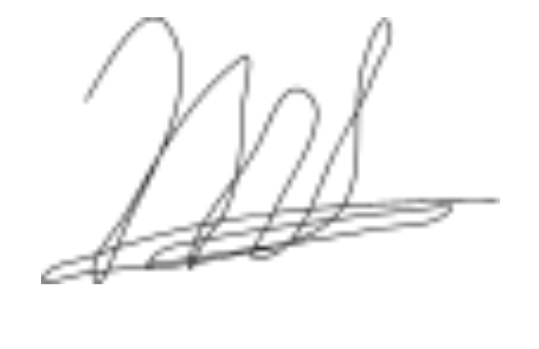
\includegraphics[width=1.5cm]{Names/Martin.png} \\
    \hline
    7106221 & Muntakim Rahman &  & 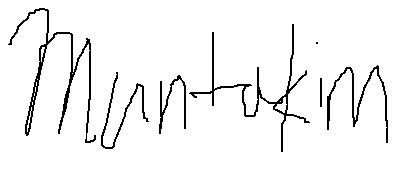
\includegraphics[width=1.5cm]{Names/Muntakim.png} \\
    \hline
    76029933 & James Huang &  & 
\includegraphics[width = 1.5cm]{Names/James.jpeg}\\
    \hline
    17542499 & Emile Jansen  &  & 
\includegraphics[width = 1.5cm]{Names/Emile.png} \\
    \hline
    46634911 & Kyden McCaskill &  & 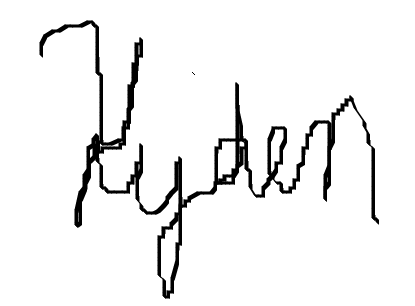
\includegraphics[width=1.5cm]{Names/Kyden.png}\\
    \hline
\end{tabular}
\end{center}

\newpage

\tableofcontents

\newpage
\section{Introduction}

\subsection{Objective}

The objective of this project was to develop a controller controlled metal-detecting robot. This was required to be
battery operated and controlled using a wireless controller. The controller is used enable smooth of control the robot's
motors; determining its direction and speed. It should also notify the user when the robot detects metal, via and LCD
display and speaker. We should be able to differentiate between the metals detected by inductance as well as sound.

\

The ultimate goal of the project is to apply the learnings from the second set of labs in this course, with two families of microcontrollers.
The circuitry used is familiar to prior in this course, but is designed to enable firmware detection of inductance with electromagnetism theory.

\subsection{System Block Diagrams}

In order to meet these system requirements and specifications, we designed the hardware and software as shown below. We will refer to this later in the report.

\begin{figure}[h]
        \centering
        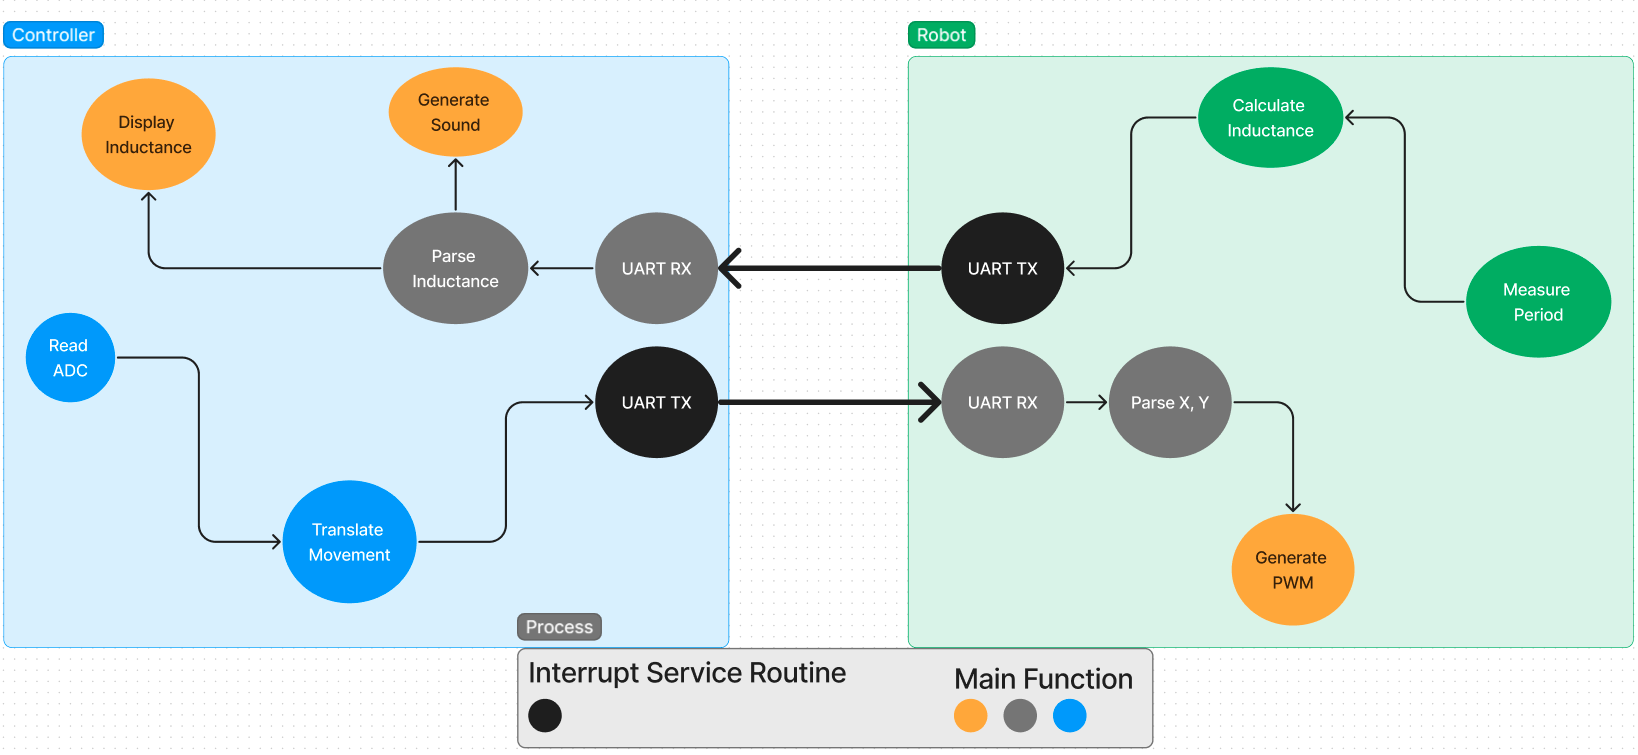
\includegraphics[width=1\linewidth]{Figures/Firmware_Block_Diagram.png}
        \caption{Firmware Block Diagram}
        \label{fig:firmware_block_diagram}
\end{figure}

\section{Investigation}

Prior to settling on a final design, we individually and collaboratively scoped out the constraints of our prroject components.

\subsection{Idea Generation}

We generated ideas for our implementation by discussing the process for meeting each of the individual specifications.
This enabled dissecting the problem into smaller and manageable parts, as well as effective task allocation for firmware and
hardware development. We discussed how each of these parts would work together to yield a fully functional robot. We prototyped individual components
in isolated test environments to confirm details, such as the functionality of the joystick and PWM peripherals, the performance of the movement logic,
and the the JDY-40transmission from one microcontroller to the next. Integrating these functional components into a functional product was the
final step, allowing us to fine-tune initial designs collaboratively through end-to-end testing.

\subsection{Investigation Design}

To begin our design, we leveraged our knowledge of Labs 4-6 to understand how sub-circuitry and software modules should be implemented. A few components required further research, such as the Colpitts Oscillator for the metal detector, and the \textit{JDY-40} radio module for data transmission.
For our circuitry, we referred to datasheets to ensure our electrical components were powered in the appropriate voltage ranges.
We also determined capacitances which would enable a stable steady state for the Colpitts Oscillator and enable us to meet expected inductance values.
For the \textit{JDY-40}, we spent some time understanding its limitations and how to properly configure it for communication between the two microcontrollers.

\subsection{Data Collection}

We collected data through extensive user testing both individually and as a group, akin to regression testing in software development.
The key process consisted of using the controller to move the robot and ensuring it met expectations. We debugged the JDY-40 communication with
\texttt{printf(tx\_data);} and \texttt{printf(rx\_data);} statements, as well as ensuring the system responded to the provided inputs.

\

Qualitative testing involved trying to smoothly maneuver the robot in the desired paths (i.e. straight line, square, figure-8, etc.) as well as testing the ability to
indicate detected metal objects (i.e. via LCD display and speaker).

\

To quantitatively measure performance, the lab equipment (i.e. oscilloscope, multimeter) was used to measure the signals and ensure they were within the expected range. This was especially useful in timing our
Interrupt Service Routines (ISRs) and ensuring that the PWM signals were generated correctly.

\subsection{Data Synthesis}

During testing, we emphasized having peer group members evaluate the performance of individual modules (i.e. movement controls, inductance detection, JDY-40 communication) to
ensure that the system was functioning as expected. The developer of the given module participated in QA testing as well, but needed feedback from others to ensure we were able to address
bugs without bias. This was especially useful in evaluating \textit{JDY-40} communication for the movement controls and inductance detection.

We also developed a \textit{Python} script to access the microcontroller \textit{COM} ports and log both the movement and inductance data shared between the microcontrollers. This enabled
us to observe both response time and accuracy betweeen transmitted and received data streams.

\begin{figure}[htbp]
    \centering
    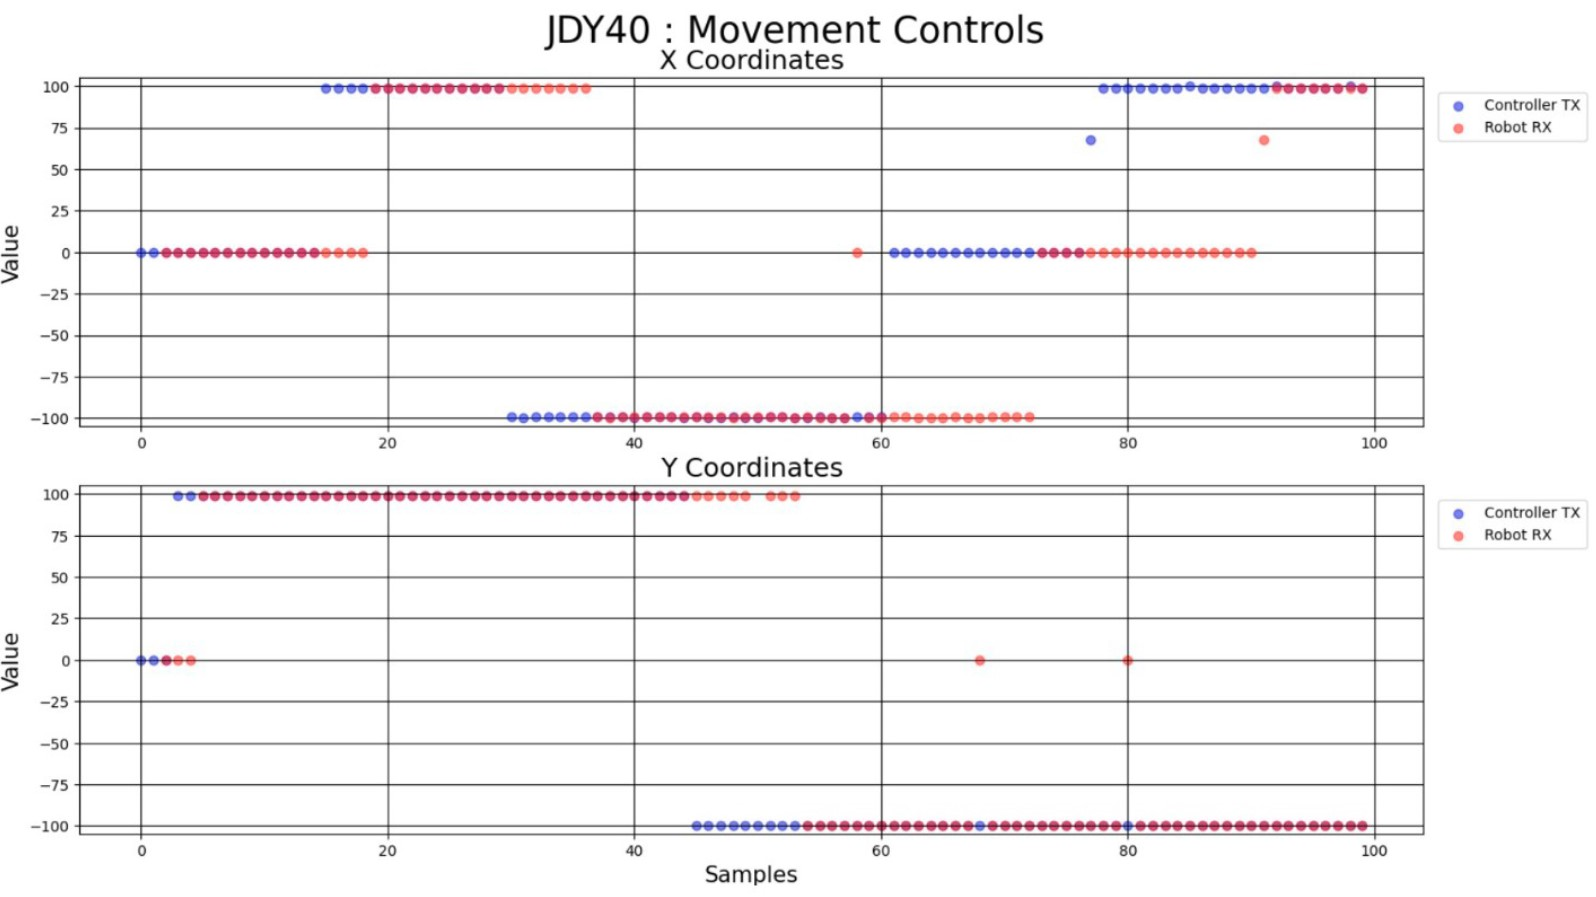
\includegraphics[width=1\textwidth]{Figures/Movement_Logs.jpg}
    \caption{Movement Controls : Data Logs}
    \label{fig:movement_controls_logs}
\end{figure}

\begin{figure}[htbp]
    \centering
    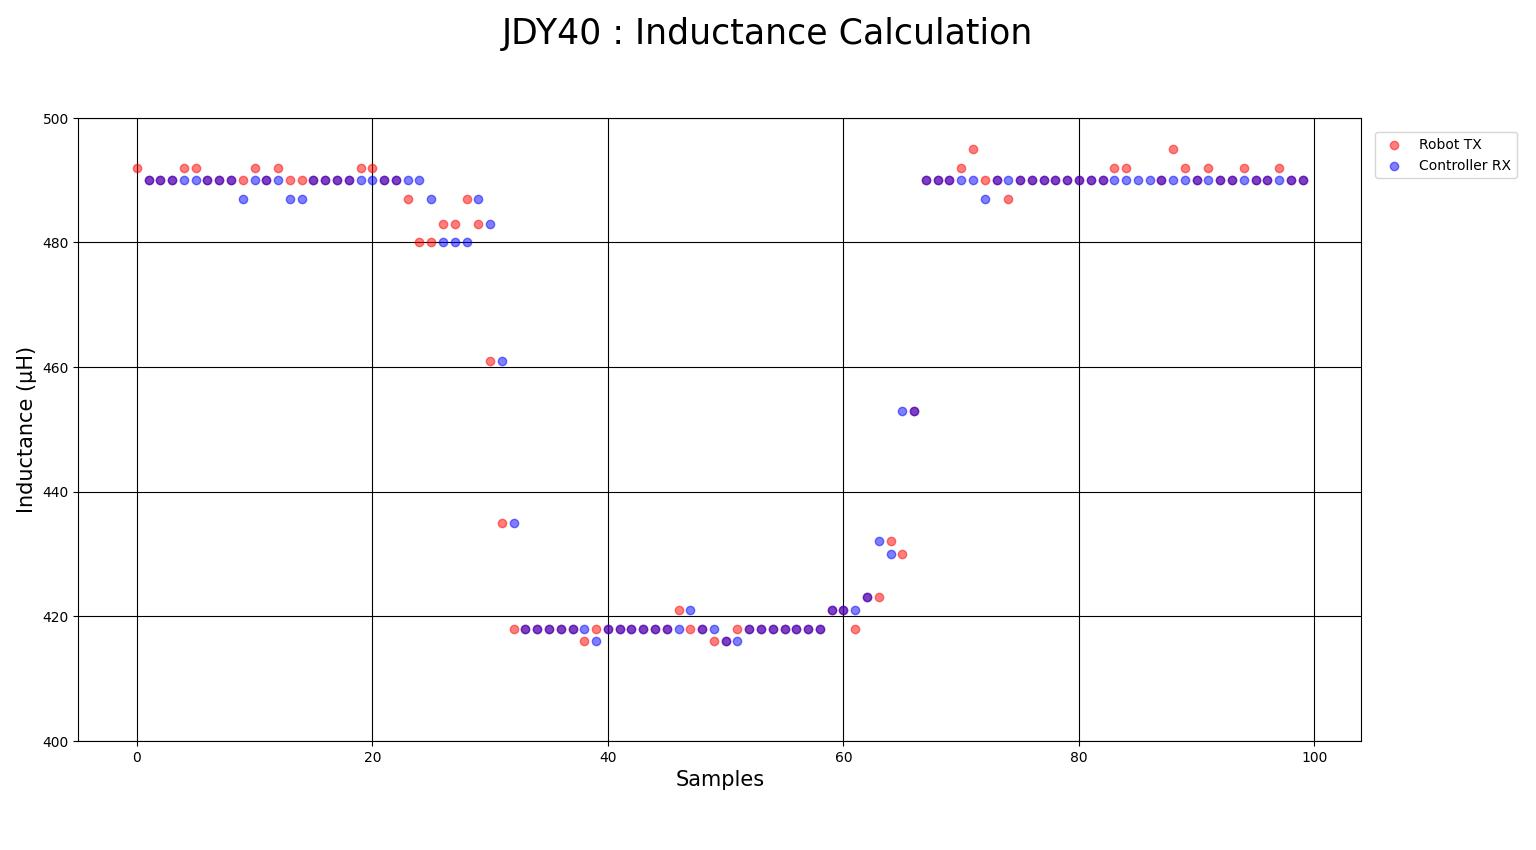
\includegraphics[width=1\textwidth]{Figures/Inductance_Logs.jpg}
    \caption{Inductance Detection : Data Logs}
    \label{fig:inductance_detection_logs}
\end{figure}

\subsection{Analysis of Results}

From the graphs above, we note that the latency is displayed as a number of samples. This was due to the fact that we had
many samples per second and wanted to visualize the microcontroller responsiveness to the change in information. From figure \ref{fig:movement_controls_logs}, we
see that the direction and speed in transmitted accurately from the \textit{STM32} to the \textit{EFM8}. In figure \ref{fig:inductance_detection_logs}, we see that the inductance values
are also transmitted accurately between the two microcontrollers. We motified both $X$ and $Y$ coordinates to test possible combinations and this was received in a reasonable number of samples.

The inductance exhibited similar behavior at the end of the development process, but we underwent many iterations on our firmware implementation to ensure that the period was
measured accurately and we were able to calculate an inductance which could be accurately used to determine magnetic thresholds. Note that it was important to be able to
bucketize inductance ranges (i.e. $400-500\, mH$, $500-600\, mH$, etc) to determine the type of metal detected.

\section{Design}

As we settled on preliminary designs of our subsystems, we required approval from team members to ensure requirements and constraints were addressed in our thought processes.

\subsection{Use of Process}

A principle we followed in development was the Work Breakdown Structure (\textit{WBS}) principle. A well planned design of individual elements ensured that we could
develop and test each module independently. This allowed us to identify and address issues in the early stages of development, and to
ensure that we can swiftly and effectively integrate building blocks into a final product.

\

Another process we emphasized was keeping track of software revisions in a well managed \textit{Git} repository. We used \textit{Visual Studio Code : Live Share}
to collaborate on the same codebase and to ensure that we were able to debug and test the code in real-time.

\

This was especially useful during dedicated group work sessions where we were adding parallel features to a \textit{development} branch. We pushed this branch to the remote repository
and merged it with the \textit{main} branch after ensuring it works exactly as intended on the microcontrollers. Tracking firmware revisions with source control also enabled quick iterations
on software modules, which helped us meet project timelines.

Requirement functionality was prioritized in the integration process, including the movement controls, inductance detection, and JDY-40 communication.
Our additional features (i.e. lock/unlock, speed limiter, turn limiter) were added after the core functionality was confirmed to be working as expected.

\subsection{Need and Constraint Identification}.

During firmware development, we identified the following constraints from the
documents provided by Dr. Jesus Calvino-Fraga[10] as well as from our own comprehension : \\
\begin{itemize}
  \item The controller and robot must be driven by two microcontrollers from different families (e.g. \textit{ARM Cortex} and \textit{8051})
  \item The robot must be able to detect metal using an inductor built from magnet wire and a coil frame.
  \item The robot must be powered by AA batteries to drive wheels and 9V for remaining functions.
  \item The speed and direction of the robot must be smoothly controlled with a joystick.
  \item The controller and the robot must wirelessly transmit data to one another.
  \item The metal detected by the robot should be indicated to the user via visual and auditory feedback.
  \item The transmission of data must be reliable and accurate.
\end{itemize}

\subsection{Problem Specification}

We quickly encountered several issues throughout the project. The main issues were the period measurements of the metal detector, JDY communications between the microcontrollers, and the overall code integration with each module.

\

\textbf{Period Measurement}
Although a seemingly trivial task, measuring a period which altered by less than 1ms was difficult to measure accurately. %continue here

\

\textbf{JDY Communications}
A key module which required extensive development time was the \textit{JDY-40} communication between the \textit{STM32} and \textit{EFM8}.
The bugs caused by this were the main blocker in integrating our firmware, as the communication was not reliable and often failed to transmit
data between the two microcontrollers. To address this challenge, we had to introduce custom timer delays instead of relying on default ones,
as the default delays blocked the execution of other code. These custom delays had to strike a balance,
ensuring they weren't excessively slow or fast. Otherwise, we risked losing data due to transmitting too quickly or rendering it obsolete
due to transmitting too slowly. We also had to ensure that the data was sent in a format that could be easily and accurately parsed by the
receiving microcontroller. A major obstacle was finding that \textit{Git} commits with a functional \textit{JDY-40} module would suddenly behave erratically
(i.e. transmission delays, inaccurate data to be received). We believe this was partially due to software bugs, but also due to the high number of \textit{JDY-40s}
in the lab environment during the latter part of the project.

\textbf{Integration}
Integrating all the code together was a major hassle. Some code that would work individually would suddenly malfunction when it was combined together.
One example of this was when we added the \textit{JDY-40} program to the speaker code on the \textit{STM32}. \dots We realized the error was that Timer 2..
Another key example was when we incorporated the \textit{JDY-40} code with the PWM code on the \textit{EFM8}, both \textit{JDY} and PWM failed due to


%mainly involving communication between the controller and the robot. The JDY-40radio functionality often was often faulty, leading to the robot and the controller being unable to transmit signals between each other. We assembled into smaller groups to collectively debug the function and ensure it's compatibility with the rest of the code.

 %We went through similar processes for balancing speed/deterministic behavior with functionality and constructing extensive circuitry for parallel functionality for the period detection, JDY-40 communication, and PWM generation.

\subsection{Solution Generation}

We found that the best way to develop our solution was through the same four-step process as in project 1. This involved : \\

\begin{enumerate}
  \item Discussing the individual requirements and assigning development to team members.
  \item Developing sub modules in a test environment.
  \item Integrating the sub modules into a single, cohesive product.
  \item Exhaustively test and debug functionality until requirements are met.
\end{enumerate}

To address recurring and ongoing issues, we relied on the \textit{WBS} principle to isolate them from the rest of our system.
This was critical in investgating the firmware issues related to the \textit{JDY-40} radio and to understand whether the transmission rate was the culprit
in unreliable and inaccurate data.

\

We initially had both \textit{UART} transmission and reception in the same \textit{ISR}, but we observed that receiving data asynchronously
caused our microcontroller to crash. We soon realized this functionality had to be synchronous and a part of the main program. However, we liked being able to control the timing of
transmission to ensure that the data was sent at a consistent rate. We also had to ensure that the data was sent in a format that could be easily parsed by the receiving microcontroller.

\

Tackling the problems in the section above in a collaborative manner allowed us to address them comprehensively and perform
testing during the development process. We also found that ownership over individual subcomponents allowed us to effectively identify the problems in the section above.

\subsection{Solution Evaluation}

To evaluate our final implementation, we emphasized

\subsection{Safety/Professionalism}

To ensure our product was safe, we developed many safety algorithms in the program. Before the robot can be controlled, the user must enter a 4 digit passcode to "unlock" the remote controller. This was paired with a lock feature which would disable the remote in the need of an emergency or other purpose.
In addition, we implemented a speed limiter and turn limiter on the remote controller for the movement of the robot. If the user wants to operate at a lower speed without the risk of too much speed, a simple click would enable this.
Furthermore, all this information was displayed on an LCD to minimize confusion and to ensure clarity. To ensure professionalism, we maintained a clean and organized codebase, and we also maintained a professional attitude in our communication and collaboration during the project.

\subsection{Detailed Design}

\subsubsection{Hardware Design}
Both the robot circuit (EFM8) and the controller circuit (STM32) were very sophisticated systems with many connections. As seen in figure \ref{fig:stm32}, the relevant circuits
include the voltage dividers, joystick (ADC), JDY-40, and LCD. Conversely, in the figure \ref{fig:efm8}, the important circuits
were the voltage dividers, JDY-40, metal detector and optocoupler/H-bridge circuits.

\

\textbf{Voltage Dividers} \\
We had a total of 4 step down voltage dividers for this project. Since the controller and the robot needed to be battery powered, we were required to use an LM7805 to drop the voltage of a standard 9V alkaline battery to 5V to power circuits such as the EFM8, LCD, speakers and the metal detector circuit. For stabilizing capacitors we used 0.22uF and 0.1uF capacitors as shown in the LM7805 datasheet. Subsequently, this 5V voltage was also dropped down to a voltage of 3v3 to power the ADC, JDY-40s and the STM32. We used 2 1uF capacitors to stabilize the signal.

\

\textbf{ADC Joystick} \\
The PS2 joystick was a basic dual ADC device to control the robot. This also did not require any complex designs as it is just two potentiometers in the x and y directions. This device was connected to 3V3 with the VRX and VRY pins connected to two ADC pins on the STM32 to measure ADC values. We also ended up using the built-in switch as a seperate button connected to a GPIO pin on the microcontroller.

\

\textbf{JDY-40 Circuit} \\
The JDY-40 (\ref{fig:JDY-40}) was used on both controller and the robot for wireless communication. The wiring was very straightforward, it was powered with 3V3 and the TX and RX pins are connected to the RX and TX pins, respectively. The SET pin was connected to a basic GPIO output on the microcontroller, used during the pairing process for AT commands (set to GND whenever an AT command needed to be sent).

\

\textbf{Metal Detector Circuit} \\
To detect metal, we used Colpitts Oscillator (\ref{fig:metaldetector}) with a discrete CMOS Inverter. This would allow us to measure a frequency related to the inductance of the inductor by using the formula $f = \frac{1}{2 \pi \sqrt{LC_T}}$, where $C_T = \frac{C_1C_2}{C_1+C_2}$. Since we wanted to use lower capacitances to allow for a larger $\Delta f$, we ended up using $C_1 =$ 1nF and $C_2 =$ 10nF. This allowed for a stable steady state and were also within the recommended range proposed by Dr. Jesus Calvino-Fraga.

\

% optocoupler and H-bridge section
\textbf{Optocoupler and H-Bridges} \\
In order to convert our voltage PWM signal into a movable operation, we needed the h-bridge and optocouplers for each motor. The H-bridges would switch the polarity of the applied voltage, enabling for forward or backwards motion depending on the strength of the applied signal. Furthermore, the contrasting high voltage operations of the motor and low voltage operations from the EMF8 is an electrical concern that we addressed by implementing the optocouplers. The optocouplers electrically isolate the two circuits, preventing voltage spikes and limiting noise, improving compatibility and efficiency. \\
Additionally, we used adequate resistors values to satisfy the 50\% current transfer ratio (CTR) and other conditions to achieve proper functionality.

\subsubsection{Firmware Design}
This project required a strong firmware foundation to ensure the robot behaved as intended. This entailed developing $C$ programs in close coordination for the \textit{STM32} and \textit{EFM8} systems.
The fundamental modules include the joystick input standardization, movement logic/PWM control, JDY-40 communications, speakers, and period calculations (metal detector).

\

\textbf{Joystick Input Standardization} \\
The raw ADC values from the joystick were not sent directly to the robot microcontroller. First, we subtracted the values by the initial ADC values they had initially (around $\frac{2^{12}-1}{2}$), to ensure when the joystick is in the middle, the value was 0.

\begin{lstlisting} [language=C, caption={Joystick Calibration}, label={lst:movementstandardized1}, basicstyle=\ttfamily\tiny]
void standardize_directions(float* x_value, float* y_value) {
    *x_value = -1 * (*x_value - X_MIDPOINT);
    *y_value = -1 * (*y_value - Y_MIDPOINT);
}
\end{lstlisting}

This was paired with some more logic to convert this number into a percentage from 1-100\% for the x and y directions. As shown in figure \ref{lst:movementstandardized2}, the value was divided by the total in the direction it was pointed to get a percent. This was paired with a minimum
 active threshold of 5\%, due to the joystick value fluctuating slightly when it was not in motion.
\begin{lstlisting} [language=C, caption={PWM Percentage Conversion}, label={lst:movementstandardized2}, basicstyle=\ttfamily\tiny]
if (y_value > MINIMUM_PERCENT_ACTIVE * (4095 - Y_MIDPOINT) || y_value < - MINIMUM_PERCENT_ACTIVE * Y_MIDPOINT) {
    if (y_value >= 0) standardized = (int)(100 * y_value / (4095 - Y_MIDPOINT));
    else if (y_value < 0) standardized = (int)(100 * y_value / (Y_MIDPOINT));
}
\end{lstlisting}

\textbf{Movement Logic/PWM Control} \\
Once the values for X and Y are sent via the JDY-40 (PWM percentages), they are inputted into the function in the listing below (\ref{lst:pwm_manager}). This logic would establish independence between the x and y values, where y would control the strength of the PWM, and x would control the percentage difference between the two wheels.

\begin{lstlisting} [language=C, caption={PWM Pulse Count Calculation}, label={lst:pwm_manager}, basicstyle=\ttfamily\tiny]
void PWM_manager(float x_value, float y_value)
{
    if (x_value >= 0) // RIGHT TURN
    {
        left_wheel = abs(y_value);
        right_wheel = (100 - abs(x_value)) * abs(y_value) / 100;
    }
    else if (x_value < 0) // LEFT TURN
    {
        left_wheel = (100 - abs(x_value)) * abs(y_value) / 100;
        right_wheel = abs(y_value);
    }
}
\end{lstlisting}

The outputted values would be counters from 0-100, which would be used for counters for the PWM duty cycles for each wheel. We ran Timer 5 at a frequency of 10kHz to allow for very precise duty cycles. The exact code for the Timer 5 ISR is in the Appendix (\ref{lst:timer5pwm}) for more details.

\

\textbf{JDY-40 Communications} \\

%Movement code ISR
%Multiple timer 0: Period
%timer 3: Delay
%timer 4: JDY
%Timer 5: PWM

%– Explain how you applied appropriate engineering knowledge,
%judgment, and tools, in creating and analyzing design solutions. This has to be
%one of biggest parts of the report. In this section you must include the description
%and evaluation of each block (e.g. “A-stable Circuit”, or “Counter Initialization”):

In order to share data between microcontrollers, we had to ensure our firmware operated deterministically and reliably.
This required ensuring that the data received by each microcontroller was accurate to the transmission and that this did not slow down the remaining functionality of the
system, especially for the robot \textit{EFM8} microcontroller.

As seen in figure \ref{fig:firmware_block_diagram}, we decided to periodically transmit data to the JDY-40 serial port module. This was done
asynchronously via ISRs. Receiving and parsing the data was done in the main function however,
as the subsequent instructions depended on a newly received value.

We prioritized frequent data transmission of movement controls from the joystick and implemented an \textit{STM32} ISR with a software counter
to transmit this every $250 ms$ via \textit{UART} communication. This ensured we can smoothly control the speed and
direction of the PWM for the robot Optocoupler and H-Bridge circuitry.

\begin{lstlisting} [language=C, caption={Timer 21 Coordinate Transmission}, label={lst:timer5pwm}, basicstyle=\ttfamily\tiny]
void TIM21_Handler(void) {
	TIM21->SR &= ~BIT0; // Clear Update Interrupt Flag
	TX21Count++;

	if (TX21Count > 250) {
		TX21Count = 0;
		TX_XY();
	}
}
\end{lstlisting}

We were able to provide slightly more leeway for transmission of inductance values, as responsiveness wasn't as time-critical as movement controls. However, we
decided to mirror the logic above on the \textit{EFM8} to send the calculated value every 250 $ms$ to the \textit{STM32}.

\textbf{Data Parsing and Validation} \\ %unbold this later


Throughout the project, we went through several prototypes for each of the functionalities and modules. Based on the learning points from previous labs and classes, we were able to implement each of the required functions into the final product.
Timer 0 was used calculating the period when detecting any change in voltage, specifically caused by the inductor passing over any metal object. Timer 3 was used for getting the delay we used throughout the overall project. Timer 4 was the timer used for programming the JDY-40and communication between the controller and the robot. Timer 5 was used for getting the PWM.

\

\textbf{Period Calculations for Metal Detector Circuit} \\
The period calculation was done with an equation that was provided to us through a piece of example code by the professor. Adjusting for the values to match our robot's characteristics, we were able to obtain accurate period readings to use later to calculate the frequency and, in turn, detect when the inductor passes over metal.

\

\textbf{Speaker} \\
%The speaker was programmed with timer 2. Using past code as reference, and by heavily modifying the values to match the robot's characteristics, we were able to operate the speaker. The defining feature of the speaker is that the output signal can increase the harmonic of the signal when in close proximity to metal. To do this, we utilised counters to keep track of which harmonic the speaker's output should be at, depending on the detected inductance values.
We implemented the speaker on the remote using timer 2 of the \textit{STM32}. We used a base frequency of 7040Hz, as this allowed us to output the perfect "A" note (sample chart shown here: \ref{fig:music_frequencies}), whereas other frequencies have decimal points (dividing the frequency by $2^n$).
In the code shown in \ref{lst:Speaker}, the \texttt{new\_ratio} value served as a counter in the Timer 2 ISR to control the PWM speed for the speaker.
The change in frequency was tied to the inductance value measured by the \textit{EFM8}.

\begin{lstlisting} [language=C, caption={Speaker control}, label={lst:Speaker}, basicstyle=\ttfamily\tiny]
float SetSpeakerFreq(float inductance_mH, float current_ratio) {
    float new_ratio, new_freq;

    // Inductance Thresholds for Speaker Frequency
    if (inductance_mH <= 435.0) new_ratio = 1;
    else if (inductance_mH < 445.0) new_ratio = 2;
    else if (inductance_mH < 455.0) new_ratio = 4;
    else if (inductance_mH < 465.0) new_ratio = 8;
    else new_ratio = 16;

    new_freq = TICK_FREQ_TIM2 / new_ratio;

    return new_ratio;
}
\end{lstlisting}



\noindent



\subsection{Solution Assessment}

We assessed our design through a set of tests.


\section{Life Long Learning}

Through this project, we gained valuable experience that would help us grow further in our respective fields of engineering. We initially encountered challenges regarding the communication between the controller and the robot, including those related to getting the JDY-40radios to communicate reliably, managing code bases for two different architectures and understanding their constraints (e.g. available timers), balancing speed/deterministic behavior with functionality, and developing extensive circuitry for parallel functionality.

On the hardware side of things, we learned how to assemble the controller and robot using multiple different microntrollers and construct the JDY-40module for radio communication. Utilizing the oscilloscope and multimeter, we were able to determine the characteristics for our firmware for those modules as well. Once again, we were able to expand upon the programming knowledge we learned in ELEC 291, CPSC 259, and CPEN 211 to program the necessary modules and integrate them into a single, cohesive product.


\section{Conclusions}
By the end of the project, we were able to develop a functional controller-controlled metal-detecting robot. The robot can move in any direction based on the input from the controller, and can transmit a signal when it detects metal, which displays information on the LCD. During our demo, it was able to determine the type and amount of coins(loonie, toonie, etc) that it detected.

In addition, we explored additional engineering principles in our feature development. This project has reinforced our skills and our foundation for future engineering projects, and was an excellent learning experience for our team.

\renewcommand{\refname}{}

\newpage

\section{References}
\begin{thebibliography}{10}


\end{thebibliography}

\clearpage
\section{Appendix}

\begin{figure}[htbp]
    \centering
    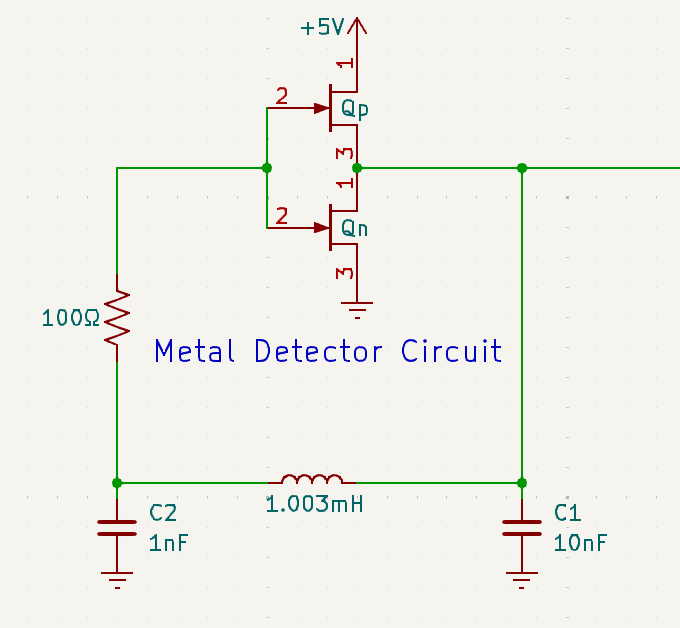
\includegraphics[width=0.5\textwidth]{Figures/metaldetector.png}
    \caption{Colpitts Oscillator with Discrete CMOS Inverter}
    \label{fig:metaldetector}
\end{figure}

\begin{figure}[htbp]
    \centering
    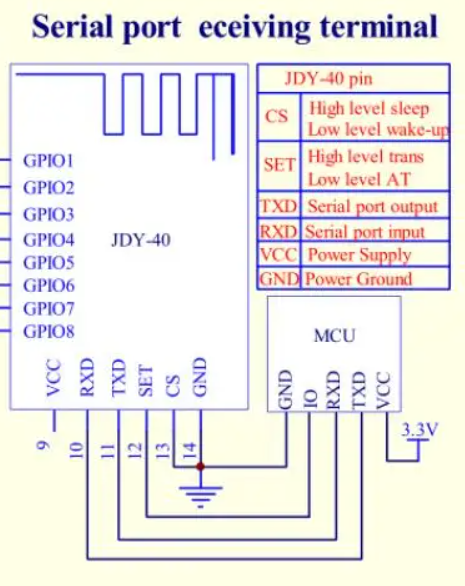
\includegraphics[width=0.3\textwidth]{Figures/jdy40.png}
    \caption{Example JDY-40 connections with a Microcontroller}
    \label{fig:JDY-40}
\end{figure}

\begin{figure}[htbp]
    \centering
    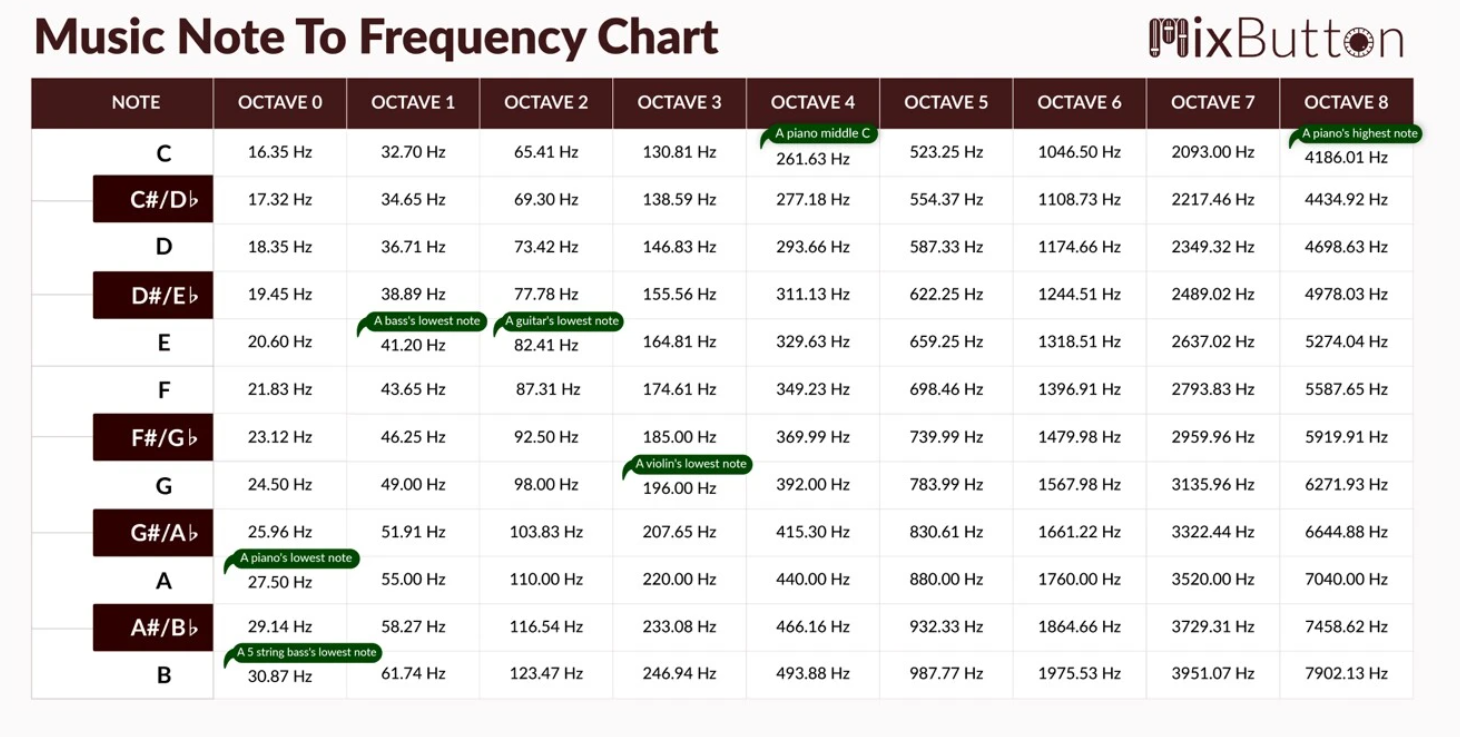
\includegraphics[width=0.3\textwidth]{Figures/Music_Frequencies.png}
    \caption{Musical Notes and their Frequencies}
    \label{fig:music_frequencies}
\end{figure}

\begin{lstlisting} [language=C, caption={Timer 5 PWM Generation}, label={lst:timer5pwm}, basicstyle=\ttfamily\tiny]
if (count > 100)
    {
        count = 0;
    }
    if (PWM_percent_y >= 0)
    {
        LEFT_MOTOR_LHS = (count > left_wheel ) ? 0:1;
        RIGHT_MOTOR_LHS = (count > new_right_wheel) ? 0:1;
    }
    else
    {
        LEFT_MOTOR_LHS = (count > left_wheel) ? 1:0;
        RIGHT_MOTOR_LHS = (count > new_right_wheel) ? 1:0;
    }

    count++;
\end{lstlisting}

\end{document}